\chapter{Scintillators} \label{ch:scintillators}
The detection of previously described particles is a key task in various applications like radiation monitoring, research and nuclear medicine. The material class of \tit{scintillators} provides candidates in diverse shapes, densities and phases for numerous requirements. In this chapter, solid scintillators are introduced.
\section{Overview}
The generation of \tit{luminescence}, emission of light with a characteristic spectrum caused by interaction of ionizing particles due to compton scattering, photoeffect and pair production (see chapter \ref{ch:particles}), is called \tit{scintillation}. 
\begin{figure}[b]
	\floatbox[{\capbeside\thisfloatsetup{capbesideposition={right,center},capbesidewidth=6.5cm}}]{figure}[\FBwidth]
	{\caption[Stokes shift]{Stokes shift for emission and absorption \cite{wermes}. The shift must be high enough to avoid re\-absorption and low enough to ideally exploit the absorption capability of the photodetector (see chapter \ref{ch:photo_detectors}).}   
		\label{fig:ch2:stokes}}
	{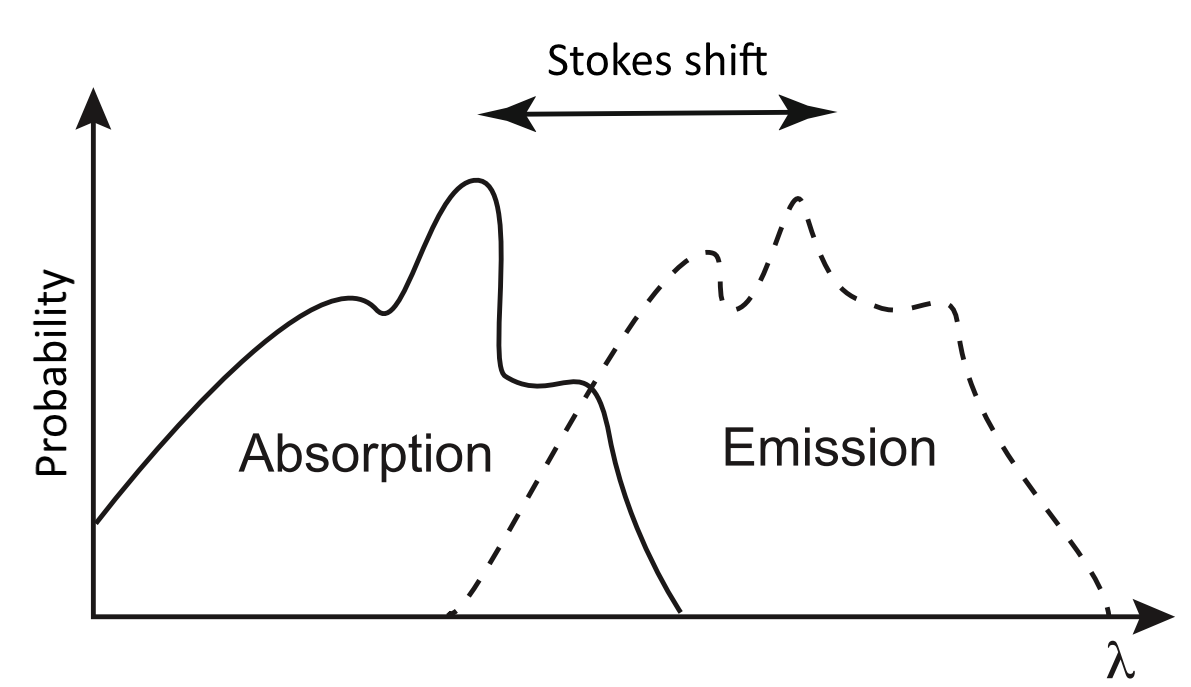
\includegraphics[width=0.5\textwidth]{./graphics/ch2/stokes.png}}
\end{figure}
The excitation, relaxation and recombination processes responsible for the emission of photons are diverse and complex, some of them will be briefly discussed later. An ideal scintillator should provide the following characteristics \cite{wermes}:
\begin{itemize}
	\setlength{\itemsep}{0pt}
	\item High \tit{light yield} (quantity of photons per energy): $L_S=\frac{<N_{ph}>}{E} \label{eq:light_yield}$. Should be proportional to the deposited energy (\tit{linearity}). 
	\item Transparency for emitted light. A high wavelength shift (\tit{Stokes shift}) to higher wavelengths for the emitted photon spectrum compared with the absorption is desired to avoid re\-absorption (see figure \ref{fig:ch2:stokes}).  
	\item Short decay time for fast response and high rates.
	\item High radiation length for full-energy measurements, low radiation length for timing.
\end{itemize}
A classical detector setup with scintillator and photodetector consists of different parts:
\begin{itemize}
	\setlength{\itemsep}{0pt}
	\item Scintillator. Must be wrapped light-tight, e.g. in Teflon foil, aluminum foil, and black tape, to keep scintillation light in and parasitic light out.
	\item \tit{Light guide.} To maximize the light output, an optical device is used to guide the scintillation light onto the photosensitive detector
	\item Photomultiplier. For the detection of scintillation light, a photomultiplier is used which can be sensitive up to single photons and provides an amplified signal.
	\item Electronics. For further amplification, a preamplifier can be used. A built-in fast discriminator can be used for timing.
\end{itemize}
\section{Organic scintillators}
The term ``organic matter" refers to carbon based materials, therefore the scintillation process of organic scintillators is dominated by electronic structures of the carbon atom. It holds six electrons (1\orb{s}{2}, 2\orb{s}{2}, 2\orb{p}{2}) and when bound in a molecule, mixed hybrid orbitals (\orb{sp}{}, \orb{sp}{2}, \orb{sp}{3}) can occur. Luminescence happens in \orb{sp}{2} and \orb{sp}{} orbitals where at least one electron is unbound (\tit{$\pi$-electron}) and the others form a strong covalent bound between the carbon atoms (\tit{$\sigma$-electrons}). \par 
The $\pi$-electron comes in singlet \stat{S}{n} and triplet states \stat{T}{n}. The main states split into vibrational states \stat{S}{ni} and \stat{T}{ni} where $n\in\mathbb{N}$ is the principle quantum number and $i\in\mathbb{N}$ is the principle quantum number of the vibrational states. A respective  \tit{Jablonski-diagram} can be found in \ref{ap:A:jablonski}. \par 
An absorption of energy leads to an excitation of the $\pi$-electron to higher states. Immediate \tit{fluorescence} is the non-radiative transition from an excited vibrational state \stat{S}{ni} to a main state \stat{S}{n0}, then, under emission of a photon, relaxation to ground state \stat{S}{00} within few nanoseconds. Radiation-free inter-system transitions from \stat{S}{ni} to \stat{T}{ni} causes \tit{phosphorescence} ($\si{\milli\second}$). \tit{Delayed fluorescence} ($\si{\milli\second}$ to $\si{\micro\second}$) is caused by a retransition from triplet state \stat{T}{1i} to \stat{S}{ni} due to thermal excitation or further ionization. These slow components have to be suppressed to grant a fast response. \par 
In order to get higher transparency and light yield, the organic scintillator consists of multiple components. A basic scintillating material (mostly \tit{polyvinyl toluene} PVT) is often mixed with a secondary scintillating material like \tit{polystyrene}, which improves light yield and response. A third component is the \tit{wavelength shifter} (WLS) which causes the necessary transparency through separating the absorption spectrum from the emission spectrum (Stokes shift). This is shown in figure \ref{fig:ch2:stokes2}. \par 
\begin{figure}[t]
	\floatbox[{\capbeside\thisfloatsetup{capbesideposition={right,center},capbesidewidth=6.5cm}}]{figure}[\FBwidth]
	{\caption[Absorption and emission of scintillator materials]{Absorption and emission spectra for different scintillator components, y-axis in arbitrary units \cite{wermes}.  PVT and p-terphenyl cover a wide absorption range of wavelengths end emit mainly in the range of the wavelength shifter \tit{POPOP}. This itself has a higher shift up to $\SI{400}{\nano\meter}$. This leads to a large stokes shift.}   
		\label{fig:ch2:stokes2}}
	{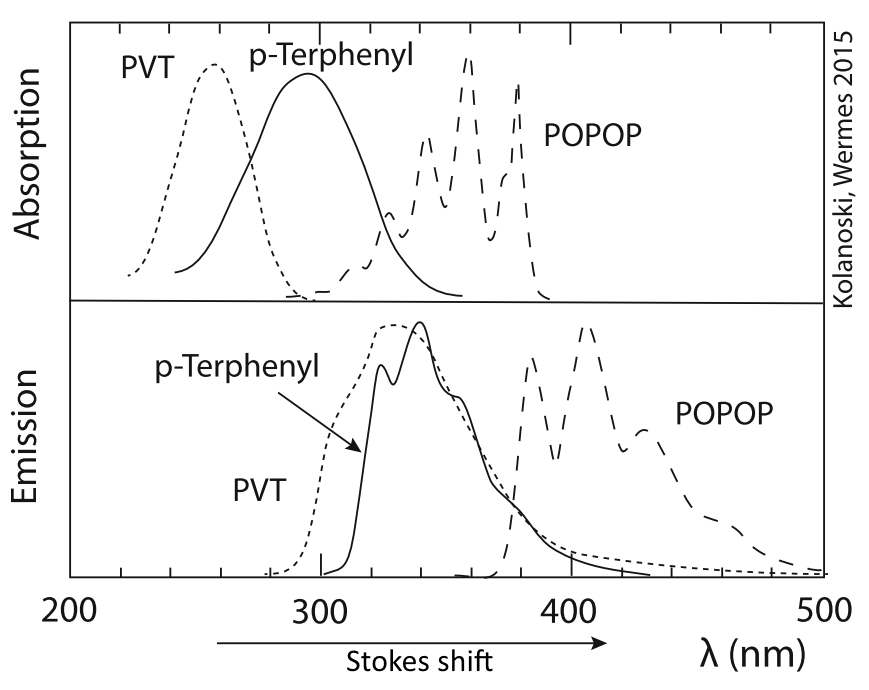
\includegraphics[width=0.5\textwidth]{./graphics/ch2/stokes2.png}}
\end{figure}
A quick coupling of three or more different components is necessary to provide sufficient speed. Between single molecules, this is done by the \tit{F\"orster resonance energy transfer} (FRET): the nonradiative excitation energy transfer by a long-range dipole dipole coupling mechanism \cite{FRET} ensures fast energy transfer from the basic material to the wavelength shifter. \par 
For minimal ionizing particles, the \tit{specific fluorescence} $\dv{S}{x}$, proportional to the light yield, can be estimated as the \tit{specific ionization} \cite{wermes}
\begin{align}
\dv{S}{r}=A\dv{E}{x}
\end{align}   
where $\dv{E}{x}$ is the specific energy loss \eqref{eq:bethe_bloch} with a proportionality factor A. For slower particles with higher energy loss, the production of quenching agents (damaged molecules) along the ionization trail of the particle has to be considered. A high ionization density deteriorates further excitation probability. The capture probability of a quenching agent relative to an undamaged molecule is given by $k_B$ (not to be confused with the Boltzmann factor). Considering this, an empirical formula, \tit{Birks law}, is given by \cite{birks}:
\begin{align}
\dv{S}{x}=\frac{A\cdot\dv{E}{x}}{1+k_B\dv{E}{X}}.
\end{align}     
For massive ionizing particles (high $\dv{E}{x}$), like fast $\alpha$-particles and heavier ions, the specific fluorescence can be described by $\dv{S}{x}=\frac{A}{k_B}$. 


\section{Inorganic scintillators}
The scintillation aspects of inorganic scintillators are given by the characteristics of the crystal lattice and electronic band structure.
\subsection{Electronic band structure} \label{ch:semiconducters} 
A \tit{crystal} is a material with a highly ordered microscopic structure, forming a lattice extending in all directions. The energy states of single atoms in the lattice are influenced by the periodic structure and form \tit{energy bands} which are separated by \tit{band gaps}. \par 
The electric conductivity is given by the two highest bands, the \tit{valence} and \tit{conduction band}. Metals in general have a good conductivity since the conduction and valence band overlap, valence electrons can directly change into the highest band and delocalize as \tit{electron gas}, providing good conductivity as free charge carriers. \tit{Semiconductors} have band gaps ranging from few hundredths of $\si{\eV}$ up to $\SI{9}{\eV}$ \cite{wermes}. \tit{Insulators} have band gaps with $>\SI{9}{\eV}$. A comparison is shown in figure \ref{fig:ch2:band_gaps}.    
\begin{figure}[b]
	\floatbox[{\capbeside\thisfloatsetup{capbesideposition={left,center},capbesidewidth=3.5cm}}]{figure}[\FBwidth]
	{\caption[Electronic band structure]{Electronic band structure for insulators (left), semiconductors (middle) and conductors (right). Amended from \cite{wermes}.}   
		\label{fig:ch2:band_gaps}}
	{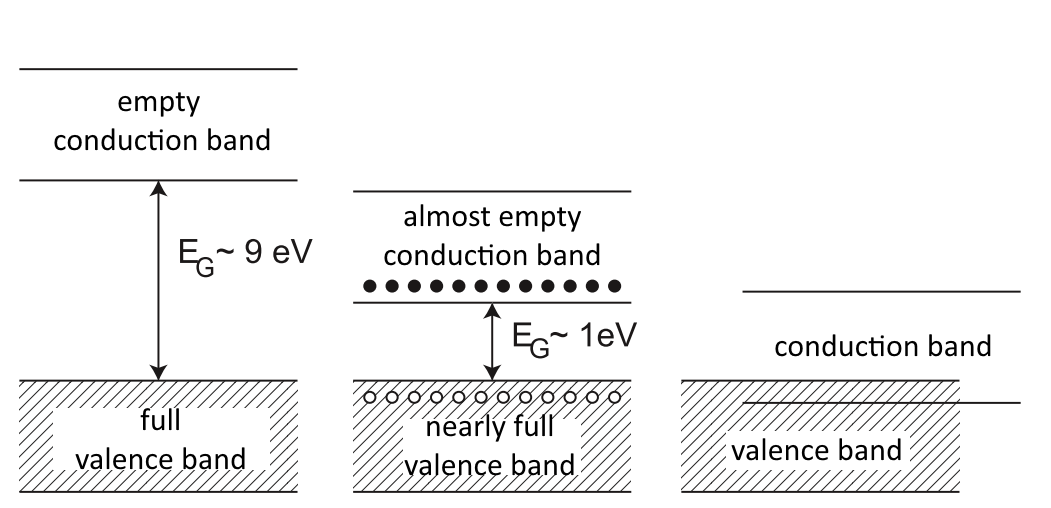
\includegraphics[width=0.75\textwidth]{./graphics/ch2/band_gaps.png}}
\end{figure}
The band gap of a scintillator lies roughly between $\SI{4}{\eV}$ and $\SI{12}{\eV}$. \par 
The creation of scintillation light is done by absorption of energy, exciting electrons from the valence band to the conduction band and relaxing back via photon emission. These processes are numerous and some will be discussed below.
\subsection{Creation of electron-hole pairs}
According to \cite{rodnyi}, the creation and annihilation of \tit{electron-hole pairs} can be separated into four stages. \par 
First, an incident particle creates and electron-hole pair by transferring energy to a bound electron, exciting it to the conduction band. The depth of the corresponding hole (usually in an inner shell) depends on the particles energy. \par 
The second stage describes the relaxation of both electrons and holes. Deep holes (in core shells) can relax by emitting radiation or nonradiative due to the \tit{Auger effect}, creating a new electron. The electron created in the first place loses energy because of inelastic electron-electron scattering. \par 
In the thermalization stage, the electrons and holes have not enough energy left for further ionization. Electrons move down to the edge of the conduction band, holes rise to the top of the valence band. \par 
The last stage describes the creation of scintillation light by excitation of \tit{luminescence centers}.
\subsection{Luminescence centers}
The energy states of the luminescence centers are smaller than the band gap of the scintillator. Hence, the optical emission spectrum is Stokes shifted to avoid reabsorption. \par 
\begin{figure}[t]
	\floatbox[{\capbeside\thisfloatsetup{capbesideposition={right,center},capbesidewidth=6.5cm}}]{figure}[\FBwidth]
	{\caption[Luminescence center]{Energy states of luminescence centers \cite{wermes}. The excitation (\ft{A}{C}) relaxes either due to thermal relaxation (\ft{C}{B}) or nonradiative transition ($F$). The luminescence transition is \ft{B}{D}. Since the energy for \ft{B}{D} is smaller than \ft{A}{C}, the emission spectrum is stokes shifted.}   
		\label{fig:ch2:luminescence}}
	{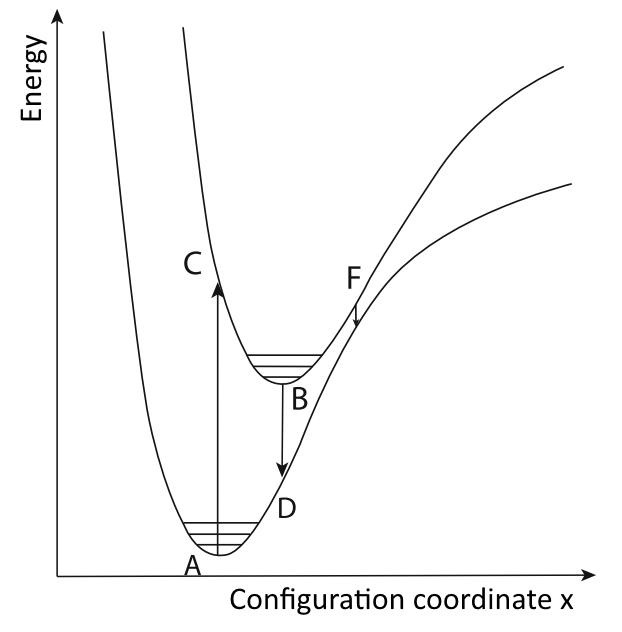
\includegraphics[width=0.5\textwidth]{./graphics/ch2/lum_center.png}}
\end{figure}
These centers can be intrinsic due to radiation damage or extrinsic by doping with activators to manipulate local electronic configurations. This improves the light yield.\par 
In figure \ref{fig:ch2:luminescence} the potential of a luminescence center is shown. Because of local polarization and thermal effects, the energy states are slightly shifted \cite{wermes}. The excitation of a center by \tit{excitons} (coupled electron-hole pairs) or absorption of electrons and holes follows the \tit{Franck-Condon principle}. It states, that transitions to corresponding vibrational states with minimal change in the nuclear number are favored \cite{franck}. This results in a higher excitation. After a thermal relaxation into the excited ground state, the center relaxes under emission of a photon. A nonradiative relaxation (quenching) is possible when the energy bands are close and thermal exchange through phonon coupling is likely. 
\subsection{Time scales}
The different time scales of the scintillation process of an intrinsic scintillator are illustrated in figure \ref{fig:ch2:time_scales} \cite{Lecoq}.
\begin{figure}[b!]
	\centering
	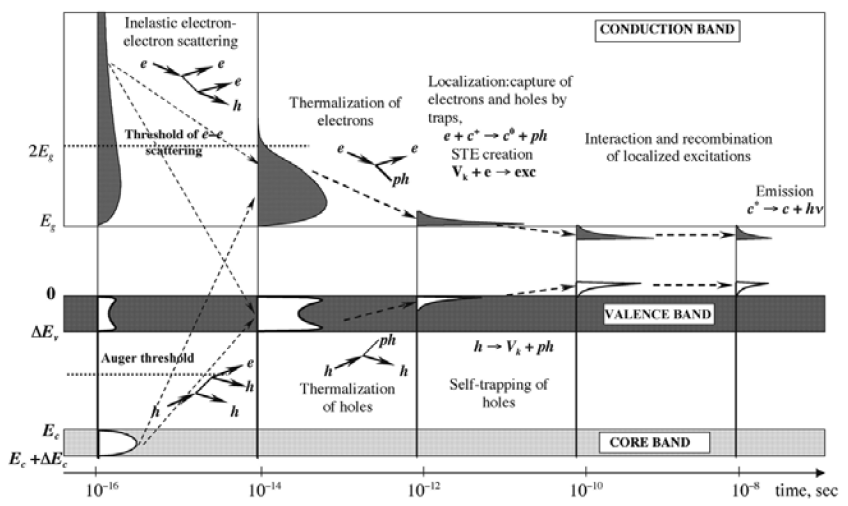
\includegraphics[width=0.85\textwidth]{./graphics/ch2/time_scales.png}
	\caption[Time scales of luminescence in inorganic scintillators]{Time scales of the scintillation process of an intrinsic organic crystal \cite{Lecoq}. Explanations can be found in the text.}   
	\label{fig:ch2:time_scales}
\end{figure}
After creating a deep core hole and exciting the corresponding electron, the energy is dissipated within $10^{-16}$ $\si{\second}$ to $10^{-14}$ $\si{\second}$ via electron-electron scattering, respectively Auger effect. Beneath a certain threshold, thermalization by phonon scattering dominates (up to $10^{-12}$ $\si{\second}$). On scales of $10^{-10}$ $\si{\second}$ to $10^{-8}$ $\si{\second}$, the charge carriers activate a luminescence center which subsequently emits scintillation light. \par     
Because of localization effects and impurities, \tit{trapping centers} can shortly trap a hole or an electron. Thermalization can release it after some hundreds of picoseconds. The thermalization of holes and excitons can be delayed by self-trapping which arises due to interaction with local phonons \cite{rodnyi}. \par
Another fast mechanism is the \tit{deep core luminescence}: if the absorption of energy creates a deep hole in the core band and the band gap between valence and conduction band is high ($>\SI{7}{\eV}$), then an ultra fast recombination (some hundred picoseconds) with a valence electron under emission of an optical photon is likely \cite{wermes}. Most of these crystals possess this fast and the conventional slow component, a prominent example being \baf.   
\section{Comparison and applications}
Since diverse applications require a variety of different properties, many scintillators have been developed. Some of the most important characteristics will be discussed. A short overview is given in table \ref{ch2:tab:characteristics}. \par 
As stated before, scintillators are produced in many different geometries. The organic plastics, above all, can be cast in various shapes. The inorganic crystals are limited in size and geometry by the growing method. Crystals are mostly produced as bars or cylinders. \par  
The speed of the scintillation process depends on the particular mechanism. Generally, plastics are faster than crystals, whereas some exceptions exist (\baf). Due to material, production process and size, the costs vary strongly. \par 
The radiation length and density are key factors for some applications. For timing purposes the particles should not be influenced, hence less dense materials, i.e. plastics, are valid. Energy measurements require a dense material able to stop particles within a small area, therefore crystals are used. \par 
The peak emission wavelength $\lambda_{em}$ and light yield are key factors for choosing an adequate photodetector. They play a crucial role in application: for timing, one needs only few photons whereby energy measurements need a great number of photons for sufficient precision. \par 
In medical applications (PET, CT), $\gamma$-spectroscopy, energy measurements in high energy physics and radiation monitoring, crystals are state-of-the-art. Plastics are often used for timing, time-of-flight measurements and detection of charged particles, e.g. cosmic rays.

\begin{table}[b]
	\centering
	\begin{tabular}{ cccccccc } \toprule[2pt]
		Material & $\rho$ [$\si{\gram}/\si{\cubic\centi\meter}$] & $\lambda_{em}$ [$\si{\nano\meter}$] & L$_{S}$ & $\tau_{decay}$ [$\si{\nano\second}$] & $\mu$ [$\si{\centi\meter}$] & $X_0$ [$\si{\centi\meter}$] & Src \\ \midrule
		EJ-248M & 1.023 & 425 & 9200 & 2.1 & 250 & $-$ &  \cite{eljen}\\
		EJ-204  & 1.023 & 408 & 10400 & 1.8 & 160 & $-$ & \cite{eljen}\\
		EJ-301  & 0.874 & 425 & 12000 & 3.2 & 3000 & $-$ & \cite{eljen} \\ 
		NaI(Tl) & 3.670 & 415 & 38000 & 250 & $-$ & 2.59 & \cite{saint-gobain} \\
		BGO & 7.130 & 480 & 10000 & 300 & $-$ & 1.14 & \cite{saint-gobain} \\
		\baf & 4.880 & 195/310 & 1800/10000 & 0.8/630 & $-$ & 2.03 & \cite{saint-gobain} \\
		LYSO & 7.100 & 420 & 30000 & 45 & $-$ & 1.20 & \cite{saint-gobain} \\
		\pwo & 8.280 & 425 & 130 & 30 & $-$ & 0.89 & \cite{wermes} \\ \bottomrule[2pt]
	\end{tabular}
	\caption[Comparison of different scintillators]{Comparison of different scintillators. The first two are plastics, the third one is liquid, the last four are solid crystals. Note that BaF$_2$ has two scintillation components. $\mu$ is the light attenuation coefficient (see \eqref{eq:beer_lambert}).}
	\label{ch2:tab:characteristics}
\end{table}





























